\documentclass[1p]{elsarticle_modified}
%\bibliographystyle{elsarticle-num}

%\usepackage[colorlinks]{hyperref}
%\usepackage{abbrmath_seonhwa} %\Abb, \Ascr, \Acal ,\Abf, \Afrak
\usepackage{amsfonts}
\usepackage{amssymb}
\usepackage{amsmath}
\usepackage{amsthm}
\usepackage{scalefnt}
\usepackage{amsbsy}
\usepackage{kotex}
\usepackage{caption}
\usepackage{subfig}
\usepackage{color}
\usepackage{graphicx}
\usepackage{xcolor} %% white, black, red, green, blue, cyan, magenta, yellow
\usepackage{float}
\usepackage{setspace}
\usepackage{hyperref}

\usepackage{tikz}
\usetikzlibrary{arrows}

\usepackage{multirow}
\usepackage{array} % fixed length table
\usepackage{hhline}

%%%%%%%%%%%%%%%%%%%%%
\makeatletter
\renewcommand*\env@matrix[1][\arraystretch]{%
	\edef\arraystretch{#1}%
	\hskip -\arraycolsep
	\let\@ifnextchar\new@ifnextchar
	\array{*\c@MaxMatrixCols c}}
\makeatother %https://tex.stackexchange.com/questions/14071/how-can-i-increase-the-line-spacing-in-a-matrix
%%%%%%%%%%%%%%%

\usepackage[normalem]{ulem}

\newcommand{\msout}[1]{\ifmmode\text{\sout{\ensuremath{#1}}}\else\sout{#1}\fi}
%SOURCE: \msout is \stkout macro in https://tex.stackexchange.com/questions/20609/strikeout-in-math-mode

\newcommand{\cancel}[1]{
	\ifmmode
	{\color{red}\msout{#1}}
	\else
	{\color{red}\sout{#1}}
	\fi
}

\newcommand{\add}[1]{
	{\color{blue}\uwave{#1}}
}

\newcommand{\replace}[2]{
	\ifmmode
	{\color{red}\msout{#1}}{\color{blue}\uwave{#2}}
	\else
	{\color{red}\sout{#1}}{\color{blue}\uwave{#2}}
	\fi
}

\newcommand{\Sol}{\mathcal{S}} %segment
\newcommand{\D}{D} %diagram
\newcommand{\A}{\mathcal{A}} %arc


%%%%%%%%%%%%%%%%%%%%%%%%%%%%%5 test

\def\sl{\operatorname{\textup{SL}}(2,\Cbb)}
\def\psl{\operatorname{\textup{PSL}}(2,\Cbb)}
\def\quan{\mkern 1mu \triangleright \mkern 1mu}

\theoremstyle{definition}
\newtheorem{thm}{Theorem}[section]
\newtheorem{prop}[thm]{Proposition}
\newtheorem{lem}[thm]{Lemma}
\newtheorem{ques}[thm]{Question}
\newtheorem{cor}[thm]{Corollary}
\newtheorem{defn}[thm]{Definition}
\newtheorem{exam}[thm]{Example}
\newtheorem{rmk}[thm]{Remark}
\newtheorem{alg}[thm]{Algorithm}

\newcommand{\I}{\sqrt{-1}}
\begin{document}

%\begin{frontmatter}
%
%\title{Boundary parabolic representations of knots up to 8 crossings}
%
%%% Group authors per affiliation:
%\author{Yunhi Cho} 
%\address{Department of Mathematics, University of Seoul, Seoul, Korea}
%\ead{yhcho@uos.ac.kr}
%
%
%\author{Seonhwa Kim} %\fnref{s_kim}}
%\address{Center for Geometry and Physics, Institute for Basic Science, Pohang, 37673, Korea}
%\ead{ryeona17@ibs.re.kr}
%
%\author{Hyuk Kim}
%\address{Department of Mathematical Sciences, Seoul National University, Seoul 08826, Korea}
%\ead{hyukkim@snu.ac.kr}
%
%\author{Seokbeom Yoon}
%\address{Department of Mathematical Sciences, Seoul National University, Seoul, 08826,  Korea}
%\ead{sbyoon15@snu.ac.kr}
%
%\begin{abstract}
%We find all boundary parabolic representation of knots up to 8 crossings.
%
%\end{abstract}
%\begin{keyword}
%    \MSC[2010] 57M25 
%\end{keyword}
%
%\end{frontmatter}

%\linenumbers
%\tableofcontents
%
\newcommand\colored[1]{\textcolor{white}{\rule[-0.35ex]{0.8em}{1.4ex}}\kern-0.8em\color{red} #1}%
%\newcommand\colored[1]{\textcolor{white}{ #1}\kern-2.17ex	\textcolor{white}{ #1}\kern-1.81ex	\textcolor{white}{ #1}\kern-2.15ex\color{red}#1	}

{\Large $\underline{12n_{0363}~(K12n_{0363})}$}

\setlength{\tabcolsep}{10pt}
\renewcommand{\arraystretch}{1.6}
\vspace{1cm}\begin{tabular}{m{100pt}>{\centering\arraybackslash}m{274pt}}
\multirow{5}{120pt}{
	\centering
	\includegraphics[width=112pt]{../../../GIT/diagram.site/Diagrams/png/2452_12n_0363.png}\\
\ \ \ A knot diagram\footnotemark}&
\allowdisplaybreaks
\textbf{Linearized knot diagam} \\
\cline{2-2}
 &
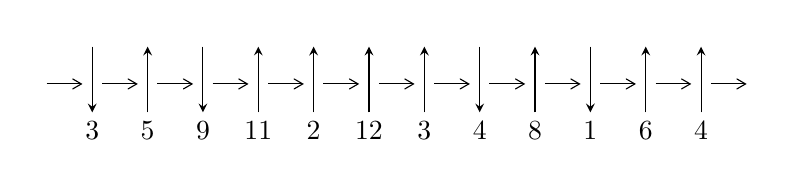
\begin{tikzpicture}[x=20pt, y=17pt]
	% nodes
	\node (C0) at (0, 0) {};
	\node (C1) at (1, 0) {};
	\node (C1U) at (1, +1) {};
	\node (C1D) at (1, -1) {3};

	\node (C2) at (2, 0) {};
	\node (C2U) at (2, +1) {};
	\node (C2D) at (2, -1) {5};

	\node (C3) at (3, 0) {};
	\node (C3U) at (3, +1) {};
	\node (C3D) at (3, -1) {9};

	\node (C4) at (4, 0) {};
	\node (C4U) at (4, +1) {};
	\node (C4D) at (4, -1) {11};

	\node (C5) at (5, 0) {};
	\node (C5U) at (5, +1) {};
	\node (C5D) at (5, -1) {2};

	\node (C6) at (6, 0) {};
	\node (C6U) at (6, +1) {};
	\node (C6D) at (6, -1) {12};

	\node (C7) at (7, 0) {};
	\node (C7U) at (7, +1) {};
	\node (C7D) at (7, -1) {3};

	\node (C8) at (8, 0) {};
	\node (C8U) at (8, +1) {};
	\node (C8D) at (8, -1) {4};

	\node (C9) at (9, 0) {};
	\node (C9U) at (9, +1) {};
	\node (C9D) at (9, -1) {8};

	\node (C10) at (10, 0) {};
	\node (C10U) at (10, +1) {};
	\node (C10D) at (10, -1) {1};

	\node (C11) at (11, 0) {};
	\node (C11U) at (11, +1) {};
	\node (C11D) at (11, -1) {6};

	\node (C12) at (12, 0) {};
	\node (C12U) at (12, +1) {};
	\node (C12D) at (12, -1) {4};
	\node (C13) at (13, 0) {};

	% arrows
	\draw[->,>={angle 60}]
	(C0) edge (C1) (C1) edge (C2) (C2) edge (C3) (C3) edge (C4) (C4) edge (C5) (C5) edge (C6) (C6) edge (C7) (C7) edge (C8) (C8) edge (C9) (C9) edge (C10) (C10) edge (C11) (C11) edge (C12) (C12) edge (C13) ;	\draw[->,>=stealth]
	(C1U) edge (C1D) (C2D) edge (C2U) (C3U) edge (C3D) (C4D) edge (C4U) (C5D) edge (C5U) (C6D) edge (C6U) (C7D) edge (C7U) (C8U) edge (C8D) (C9D) edge (C9U) (C10U) edge (C10D) (C11D) edge (C11U) (C12D) edge (C12U) ;
	\end{tikzpicture} \\
\hhline{~~} \\& 
\textbf{Solving Sequence} \\ \cline{2-2} 
 &
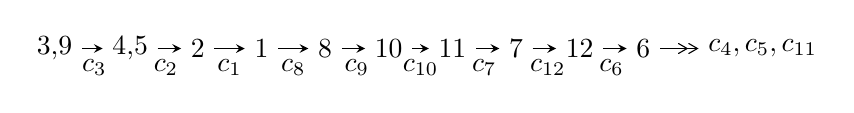
\begin{tikzpicture}[x=23pt, y=7pt]
	% node
	\node (A0) at (-1/8, 0) {3,9};
	\node (A1) at (17/16, 0) {4,5};
	\node (A2) at (17/8, 0) {2};
	\node (A3) at (25/8, 0) {1};
	\node (A4) at (33/8, 0) {8};
	\node (A5) at (41/8, 0) {10};
	\node (A6) at (49/8, 0) {11};
	\node (A7) at (57/8, 0) {7};
	\node (A8) at (65/8, 0) {12};
	\node (A9) at (73/8, 0) {6};
	\node (C1) at (1/2, -1) {$c_{3}$};
	\node (C2) at (13/8, -1) {$c_{2}$};
	\node (C3) at (21/8, -1) {$c_{1}$};
	\node (C4) at (29/8, -1) {$c_{8}$};
	\node (C5) at (37/8, -1) {$c_{9}$};
	\node (C6) at (45/8, -1) {$c_{10}$};
	\node (C7) at (53/8, -1) {$c_{7}$};
	\node (C8) at (61/8, -1) {$c_{12}$};
	\node (C9) at (69/8, -1) {$c_{6}$};
	\node (A10) at (11, 0) {$c_{4},c_{5},c_{11}$};

	% edge
	\draw[->,>=stealth]	
	(A0) edge (A1) (A1) edge (A2) (A2) edge (A3) (A3) edge (A4) (A4) edge (A5) (A5) edge (A6) (A6) edge (A7) (A7) edge (A8) (A8) edge (A9) ;
	\draw[->>,>={angle 60}]	
	(A9) edge (A10);
\end{tikzpicture} \\ 

\end{tabular} \\

\footnotetext{
The image of knot diagram is generated by the software ``\textbf{Draw programme}" developed by Andrew Bartholomew(\url{http://www.layer8.co.uk/maths/draw/index.htm\#Running-draw}), where we modified some parts for our purpose(\url{https://github.com/CATsTAILs/LinksPainter}).
}\phantom \\ \newline 
\centering \textbf{Ideals for irreducible components\footnotemark of $X_{\text{par}}$} 
 
\begin{align*}
I^u_{1}&=\langle 
1.18536\times10^{82} u^{64}+1.17821\times10^{82} u^{63}+\cdots+4.44686\times10^{81} b+5.58068\times10^{82},\\
\phantom{I^u_{1}}&\phantom{= \langle  }-3.67200\times10^{85} u^{64}-4.79998\times10^{85} u^{63}+\cdots+2.88601\times10^{84} a-5.33132\times10^{86},\\
\phantom{I^u_{1}}&\phantom{= \langle  }u^{65}+u^{64}+\cdots+32 u+11\rangle \\
I^u_{2}&=\langle 
u^{16}+u^{15}+\cdots+b+2,\\
\phantom{I^u_{2}}&\phantom{= \langle  }- u^{16}- u^{15}-3 u^{14}-3 u^{13}-7 u^{12}-7 u^{11}-9 u^{10}-11 u^9-9 u^8-15 u^7-2 u^6-14 u^5-10 u^3+a-4 u-2,\\
\phantom{I^u_{2}}&\phantom{= \langle  }u^{18}+4 u^{16}+\cdots- u+1\rangle \\
I^u_{3}&=\langle 
b- u,\;u^2+a+1,\;u^4+u^2+u+1\rangle \\
\\
\end{align*}
\raggedright * 3 irreducible components of $\dim_{\mathbb{C}}=0$, with total 87 representations.\\
\footnotetext{All coefficients of polynomials are rational numbers. But the coefficients are sometimes approximated in decimal forms when there is not enough margin.}
\newpage
\renewcommand{\arraystretch}{1}
\centering \section*{I. $I^u_{1}= \langle 1.19\times10^{82} u^{64}+1.18\times10^{82} u^{63}+\cdots+4.45\times10^{81} b+5.58\times10^{82},\;-3.67\times10^{85} u^{64}-4.80\times10^{85} u^{63}+\cdots+2.89\times10^{84} a-5.33\times10^{86},\;u^{65}+u^{64}+\cdots+32 u+11 \rangle$}
\flushleft \textbf{(i) Arc colorings}\\
\begin{tabular}{m{7pt} m{180pt} m{7pt} m{180pt} }
\flushright $a_{3}=$&$\begin{pmatrix}1\\0\end{pmatrix}$ \\
\flushright $a_{9}=$&$\begin{pmatrix}0\\u\end{pmatrix}$ \\
\flushright $a_{4}=$&$\begin{pmatrix}1\\u^2\end{pmatrix}$ \\
\flushright $a_{5}=$&$\begin{pmatrix}12.7234 u^{64}+16.6319 u^{63}+\cdots+952.459 u+184.730\\-2.66560 u^{64}-2.64952 u^{63}+\cdots-136.076 u-12.5497\end{pmatrix}$ \\
\flushright $a_{2}=$&$\begin{pmatrix}-4.71664 u^{64}+3.37825 u^{63}+\cdots+545.587 u+271.508\\0.928296 u^{64}-2.05851 u^{63}+\cdots-225.100 u-104.728\end{pmatrix}$ \\
\flushright $a_{1}=$&$\begin{pmatrix}-3.78835 u^{64}+1.31974 u^{63}+\cdots+320.487 u+166.781\\0.928296 u^{64}-2.05851 u^{63}+\cdots-225.100 u-104.728\end{pmatrix}$ \\
\flushright $a_{8}=$&$\begin{pmatrix}u\\u^3+u\end{pmatrix}$ \\
\flushright $a_{10}=$&$\begin{pmatrix}u^3\\u^5+u^3+u\end{pmatrix}$ \\
\flushright $a_{11}=$&$\begin{pmatrix}6.96248 u^{64}+13.4113 u^{63}+\cdots+961.700 u+259.286\\-2.60048 u^{64}-3.57741 u^{63}+\cdots-231.000 u-51.3320\end{pmatrix}$ \\
\flushright $a_{7}=$&$\begin{pmatrix}- u^3\\u^3+u\end{pmatrix}$ \\
\flushright $a_{12}=$&$\begin{pmatrix}-3.79507 u^{64}+2.51346 u^{63}+\cdots+423.800 u+215.319\\0.628384 u^{64}-2.58932 u^{63}+\cdots-263.440 u-117.933\end{pmatrix}$ \\
\flushright $a_{6}=$&$\begin{pmatrix}1.94949 u^{64}+5.30850 u^{63}+\cdots+457.040 u+133.508\\3.65785 u^{64}+4.57938 u^{63}+\cdots+244.609 u+51.0970\end{pmatrix}$\\&\end{tabular}
\flushleft \textbf{(ii) Obstruction class $= -1$}\\~\\
\flushleft \textbf{(iii) Cusp Shapes $= -9.85489 u^{64}-0.506938 u^{63}+\cdots+295.659 u+281.817$}\\~\\
\newpage\renewcommand{\arraystretch}{1}
\flushleft \textbf{(iv) u-Polynomials at the component}\newline \\
\begin{tabular}{m{50pt}|m{274pt}}
Crossings & \hspace{64pt}u-Polynomials at each crossing \\
\hline $$\begin{aligned}c_{1}\end{aligned}$$&$\begin{aligned}
&u^{65}+36 u^{64}+\cdots-31 u-1
\end{aligned}$\\
\hline $$\begin{aligned}c_{2},c_{5}\end{aligned}$$&$\begin{aligned}
&u^{65}+18 u^{63}+\cdots+u-1
\end{aligned}$\\
\hline $$\begin{aligned}c_{3},c_{8}\end{aligned}$$&$\begin{aligned}
&u^{65}- u^{64}+\cdots+32 u-11
\end{aligned}$\\
\hline $$\begin{aligned}c_{4}\end{aligned}$$&$\begin{aligned}
&u^{65}- u^{64}+\cdots+170 u-99
\end{aligned}$\\
\hline $$\begin{aligned}c_{6},c_{11}\end{aligned}$$&$\begin{aligned}
&u^{65}- u^{64}+\cdots-290 u-374
\end{aligned}$\\
\hline $$\begin{aligned}c_{7}\end{aligned}$$&$\begin{aligned}
&u^{65}+u^{64}+\cdots-146235740 u-28512220
\end{aligned}$\\
\hline $$\begin{aligned}c_{9}\end{aligned}$$&$\begin{aligned}
&u^{65}-17 u^{64}+\cdots-3200 u+121
\end{aligned}$\\
\hline $$\begin{aligned}c_{10}\end{aligned}$$&$\begin{aligned}
&u^{65}-5 u^{64}+\cdots+404554 u-19583
\end{aligned}$\\
\hline $$\begin{aligned}c_{12}\end{aligned}$$&$\begin{aligned}
&u^{65}+3 u^{64}+\cdots+761476 u+2099
\end{aligned}$\\
\hline
\end{tabular}\\~\\
\newpage\renewcommand{\arraystretch}{1}
\flushleft \textbf{(v) Riley Polynomials at the component}\newline \\
\begin{tabular}{m{50pt}|m{274pt}}
Crossings & \hspace{64pt}Riley Polynomials at each crossing \\
\hline $$\begin{aligned}c_{1}\end{aligned}$$&$\begin{aligned}
&y^{65}+48 y^{63}+\cdots+185 y-1
\end{aligned}$\\
\hline $$\begin{aligned}c_{2},c_{5}\end{aligned}$$&$\begin{aligned}
&y^{65}+36 y^{64}+\cdots-31 y-1
\end{aligned}$\\
\hline $$\begin{aligned}c_{3},c_{8}\end{aligned}$$&$\begin{aligned}
&y^{65}+17 y^{64}+\cdots-3200 y-121
\end{aligned}$\\
\hline $$\begin{aligned}c_{4}\end{aligned}$$&$\begin{aligned}
&y^{65}-23 y^{64}+\cdots-12086 y-9801
\end{aligned}$\\
\hline $$\begin{aligned}c_{6},c_{11}\end{aligned}$$&$\begin{aligned}
&y^{65}-27 y^{64}+\cdots+1737928 y-139876
\end{aligned}$\\
\hline $$\begin{aligned}c_{7}\end{aligned}$$&$\begin{aligned}
&y^{65}+129 y^{64}+\cdots-36644682510257400 y-812946689328400
\end{aligned}$\\
\hline $$\begin{aligned}c_{9}\end{aligned}$$&$\begin{aligned}
&y^{65}+73 y^{64}+\cdots+504824 y-14641
\end{aligned}$\\
\hline $$\begin{aligned}c_{10}\end{aligned}$$&$\begin{aligned}
&y^{65}-77 y^{64}+\cdots+2489974016 y-383493889
\end{aligned}$\\
\hline $$\begin{aligned}c_{12}\end{aligned}$$&$\begin{aligned}
&y^{65}+75 y^{64}+\cdots+597043930640 y-4405801
\end{aligned}$\\
\hline
\end{tabular}\\~\\
\newpage\flushleft \textbf{(vi) Complex Volumes and Cusp Shapes}
$$\begin{array}{c|c|c}  
\text{Solutions to }I^u_{1}& \I (\text{vol} + \sqrt{-1}CS) & \text{Cusp shape}\\
 \hline 
\begin{aligned}
u &= \phantom{-}0.680009 + 0.713106 I \\
a &= \phantom{-}1.41460 + 0.20948 I \\
b &= -0.829559 + 0.897240 I\end{aligned}
 & \phantom{-}1.19074 - 3.17057 I & \phantom{-}4.00000 + 2.82300 I \\ \hline\begin{aligned}
u &= \phantom{-}0.680009 - 0.713106 I \\
a &= \phantom{-}1.41460 - 0.20948 I \\
b &= -0.829559 - 0.897240 I\end{aligned}
 & \phantom{-}1.19074 + 3.17057 I & \phantom{-}4.00000 - 2.82300 I \\ \hline\begin{aligned}
u &= -0.130389 + 1.036020 I \\
a &= \phantom{-}2.29843 + 0.93843 I \\
b &= -0.322430 - 0.884795 I\end{aligned}
 & -1.18726 + 1.38317 I & \phantom{-0.000000 } 0 \\ \hline\begin{aligned}
u &= -0.130389 - 1.036020 I \\
a &= \phantom{-}2.29843 - 0.93843 I \\
b &= -0.322430 + 0.884795 I\end{aligned}
 & -1.18726 - 1.38317 I & \phantom{-0.000000 } 0 \\ \hline\begin{aligned}
u &= \phantom{-}0.686817 + 0.660938 I \\
a &= \phantom{-}0.484110 + 0.485186 I \\
b &= -0.417093 + 1.257930 I\end{aligned}
 & \phantom{-}0.11513 - 5.57520 I & \phantom{-}1.42711 + 8.53371 I \\ \hline\begin{aligned}
u &= \phantom{-}0.686817 - 0.660938 I \\
a &= \phantom{-}0.484110 - 0.485186 I \\
b &= -0.417093 - 1.257930 I\end{aligned}
 & \phantom{-}0.11513 + 5.57520 I & \phantom{-}1.42711 - 8.53371 I \\ \hline\begin{aligned}
u &= -0.600257 + 0.736464 I \\
a &= -2.35238 + 0.68378 I \\
b &= \phantom{-}0.696793 + 0.978880 I\end{aligned}
 & \phantom{-}0.90319 + 6.82193 I & \phantom{-}4.00000 - 10.20078 I \\ \hline\begin{aligned}
u &= -0.600257 - 0.736464 I \\
a &= -2.35238 - 0.68378 I \\
b &= \phantom{-}0.696793 - 0.978880 I\end{aligned}
 & \phantom{-}0.90319 - 6.82193 I & \phantom{-}4.00000 + 10.20078 I \\ \hline\begin{aligned}
u &= \phantom{-}0.536349 + 0.783362 I \\
a &= -0.292753 - 1.310400 I \\
b &= \phantom{-}0.714251 + 0.738621 I\end{aligned}
 & \phantom{-}1.65196 - 1.37503 I & \phantom{-}5.70343 + 4.32793 I \\ \hline\begin{aligned}
u &= \phantom{-}0.536349 - 0.783362 I \\
a &= -0.292753 + 1.310400 I \\
b &= \phantom{-}0.714251 - 0.738621 I\end{aligned}
 & \phantom{-}1.65196 + 1.37503 I & \phantom{-}5.70343 - 4.32793 I\\
 \hline 
 \end{array}$$\newpage$$\begin{array}{c|c|c}  
\text{Solutions to }I^u_{1}& \I (\text{vol} + \sqrt{-1}CS) & \text{Cusp shape}\\
 \hline 
\begin{aligned}
u &= \phantom{-}0.536653 + 0.910218 I \\
a &= \phantom{-}1.30688 - 0.94688 I \\
b &= \phantom{-}0.277844 + 1.051000 I\end{aligned}
 & \phantom{-}1.022910 + 0.885443 I & \phantom{-0.000000 } 0 \\ \hline\begin{aligned}
u &= \phantom{-}0.536653 - 0.910218 I \\
a &= \phantom{-}1.30688 + 0.94688 I \\
b &= \phantom{-}0.277844 - 1.051000 I\end{aligned}
 & \phantom{-}1.022910 - 0.885443 I & \phantom{-0.000000 } 0 \\ \hline\begin{aligned}
u &= \phantom{-}0.919266 + 0.044023 I \\
a &= \phantom{-}0.685246 - 0.197964 I \\
b &= -0.400619 - 1.148570 I\end{aligned}
 & -1.32773 + 3.65915 I & \phantom{-}0.21562 - 3.87323 I \\ \hline\begin{aligned}
u &= \phantom{-}0.919266 - 0.044023 I \\
a &= \phantom{-}0.685246 + 0.197964 I \\
b &= -0.400619 + 1.148570 I\end{aligned}
 & -1.32773 - 3.65915 I & \phantom{-}0.21562 + 3.87323 I \\ \hline\begin{aligned}
u &= -0.498707 + 0.773383 I \\
a &= \phantom{-}0.440300 - 0.516252 I \\
b &= -0.706622 + 0.898570 I\end{aligned}
 & \phantom{-}1.13961 - 2.56713 I & \phantom{-}4.00000 + 1.86590 I \\ \hline\begin{aligned}
u &= -0.498707 - 0.773383 I \\
a &= \phantom{-}0.440300 + 0.516252 I \\
b &= -0.706622 - 0.898570 I\end{aligned}
 & \phantom{-}1.13961 + 2.56713 I & \phantom{-}4.00000 - 1.86590 I \\ \hline\begin{aligned}
u &= -0.714171 + 0.556638 I \\
a &= \phantom{-}0.58411 + 1.77271 I \\
b &= \phantom{-}0.158903 + 0.735534 I\end{aligned}
 & \phantom{-}2.30751 + 1.23537 I & \phantom{-}1.43112 - 2.75975 I \\ \hline\begin{aligned}
u &= -0.714171 - 0.556638 I \\
a &= \phantom{-}0.58411 - 1.77271 I \\
b &= \phantom{-}0.158903 - 0.735534 I\end{aligned}
 & \phantom{-}2.30751 - 1.23537 I & \phantom{-}1.43112 + 2.75975 I \\ \hline\begin{aligned}
u &= -0.339089 + 1.140750 I \\
a &= -1.67737 + 0.59115 I \\
b &= \phantom{-}0.628783 - 0.316202 I\end{aligned}
 & \phantom{-}5.30182 + 3.74007 I & \phantom{-0.000000 } 0 \\ \hline\begin{aligned}
u &= -0.339089 - 1.140750 I \\
a &= -1.67737 - 0.59115 I \\
b &= \phantom{-}0.628783 + 0.316202 I\end{aligned}
 & \phantom{-}5.30182 - 3.74007 I & \phantom{-0.000000 } 0\\
 \hline 
 \end{array}$$\newpage$$\begin{array}{c|c|c}  
\text{Solutions to }I^u_{1}& \I (\text{vol} + \sqrt{-1}CS) & \text{Cusp shape}\\
 \hline 
\begin{aligned}
u &= \phantom{-}0.953198 + 0.755841 I \\
a &= -0.598616 + 0.308645 I \\
b &= \phantom{-}0.445402 + 1.166070 I\end{aligned}
 & -8.89416 + 1.07478 I & \phantom{-0.000000 } 0 \\ \hline\begin{aligned}
u &= \phantom{-}0.953198 - 0.755841 I \\
a &= -0.598616 - 0.308645 I \\
b &= \phantom{-}0.445402 - 1.166070 I\end{aligned}
 & -8.89416 - 1.07478 I & \phantom{-0.000000 } 0 \\ \hline\begin{aligned}
u &= -0.854923 + 0.866674 I \\
a &= -0.496614 + 0.011802 I \\
b &= \phantom{-}0.545772 + 0.013538 I\end{aligned}
 & -5.80014 + 2.95712 I & \phantom{-0.000000 } 0 \\ \hline\begin{aligned}
u &= -0.854923 - 0.866674 I \\
a &= -0.496614 - 0.011802 I \\
b &= \phantom{-}0.545772 - 0.013538 I\end{aligned}
 & -5.80014 - 2.95712 I & \phantom{-0.000000 } 0 \\ \hline\begin{aligned}
u &= -0.833013 + 0.906851 I \\
a &= \phantom{-}0.242257 - 0.165490 I \\
b &= -0.027191 - 0.303343 I\end{aligned}
 & -5.70705 + 3.10651 I & \phantom{-0.000000 } 0 \\ \hline\begin{aligned}
u &= -0.833013 - 0.906851 I \\
a &= \phantom{-}0.242257 + 0.165490 I \\
b &= -0.027191 + 0.303343 I\end{aligned}
 & -5.70705 - 3.10651 I & \phantom{-0.000000 } 0 \\ \hline\begin{aligned}
u &= -0.549089 + 1.115550 I \\
a &= -1.74225 + 0.41891 I \\
b &= \phantom{-}0.160584 + 0.669882 I\end{aligned}
 & \phantom{-}4.17437 + 3.71139 I & \phantom{-0.000000 } 0 \\ \hline\begin{aligned}
u &= -0.549089 - 1.115550 I \\
a &= -1.74225 - 0.41891 I \\
b &= \phantom{-}0.160584 - 0.669882 I\end{aligned}
 & \phantom{-}4.17437 - 3.71139 I & \phantom{-0.000000 } 0 \\ \hline\begin{aligned}
u &= -0.797232 + 0.958267 I \\
a &= \phantom{-}0.498877 - 0.859914 I \\
b &= -0.507934 + 0.279262 I\end{aligned}
 & -5.49508 + 3.22478 I & \phantom{-0.000000 } 0 \\ \hline\begin{aligned}
u &= -0.797232 - 0.958267 I \\
a &= \phantom{-}0.498877 + 0.859914 I \\
b &= -0.507934 - 0.279262 I\end{aligned}
 & -5.49508 - 3.22478 I & \phantom{-0.000000 } 0\\
 \hline 
 \end{array}$$\newpage$$\begin{array}{c|c|c}  
\text{Solutions to }I^u_{1}& \I (\text{vol} + \sqrt{-1}CS) & \text{Cusp shape}\\
 \hline 
\begin{aligned}
u &= \phantom{-}0.447329 + 1.169880 I \\
a &= -0.453069 - 1.212100 I \\
b &= \phantom{-}0.452862 + 1.045590 I\end{aligned}
 & \phantom{-}2.40731 - 0.69677 I & \phantom{-0.000000 } 0 \\ \hline\begin{aligned}
u &= \phantom{-}0.447329 - 1.169880 I \\
a &= -0.453069 + 1.212100 I \\
b &= \phantom{-}0.452862 - 1.045590 I\end{aligned}
 & \phantom{-}2.40731 + 0.69677 I & \phantom{-0.000000 } 0 \\ \hline\begin{aligned}
u &= \phantom{-}0.950733 + 0.838002 I \\
a &= \phantom{-}1.046540 + 0.328040 I \\
b &= -1.080450 + 0.250407 I\end{aligned}
 & -3.94832 + 2.68251 I & \phantom{-0.000000 } 0 \\ \hline\begin{aligned}
u &= \phantom{-}0.950733 - 0.838002 I \\
a &= \phantom{-}1.046540 - 0.328040 I \\
b &= -1.080450 - 0.250407 I\end{aligned}
 & -3.94832 - 2.68251 I & \phantom{-0.000000 } 0 \\ \hline\begin{aligned}
u &= \phantom{-}0.023056 + 0.722524 I \\
a &= -1.76080 + 3.14396 I \\
b &= \phantom{-}0.630679 - 0.948352 I\end{aligned}
 & \phantom{-}3.75759 - 4.41575 I & \phantom{-}12.04885 + 5.91677 I \\ \hline\begin{aligned}
u &= \phantom{-}0.023056 - 0.722524 I \\
a &= -1.76080 - 3.14396 I \\
b &= \phantom{-}0.630679 + 0.948352 I\end{aligned}
 & \phantom{-}3.75759 + 4.41575 I & \phantom{-}12.04885 - 5.91677 I \\ \hline\begin{aligned}
u &= -0.713686\phantom{ +0.000000I} \\
a &= \phantom{-}1.13925\phantom{ +0.000000I} \\
b &= -0.584356\phantom{ +0.000000I}\end{aligned}
 & \phantom{-}1.80251\phantom{ +0.000000I} & \phantom{-}5.12800\phantom{ +0.000000I} \\ \hline\begin{aligned}
u &= -0.193742 + 0.683841 I \\
a &= \phantom{-}0.962945 + 0.999475 I \\
b &= -0.922328 - 0.420825 I\end{aligned}
 & \phantom{-}5.03052 + 1.51034 I & \phantom{-}15.7178 - 3.9613 I \\ \hline\begin{aligned}
u &= -0.193742 - 0.683841 I \\
a &= \phantom{-}0.962945 - 0.999475 I \\
b &= -0.922328 + 0.420825 I\end{aligned}
 & \phantom{-}5.03052 - 1.51034 I & \phantom{-}15.7178 + 3.9613 I \\ \hline\begin{aligned}
u &= -1.024200 + 0.791302 I \\
a &= \phantom{-}0.552140 - 0.058409 I \\
b &= -0.63656 + 1.26921 I\end{aligned}
 & -7.10877 - 8.80138 I & \phantom{-0.000000 } 0\\
 \hline 
 \end{array}$$\newpage$$\begin{array}{c|c|c}  
\text{Solutions to }I^u_{1}& \I (\text{vol} + \sqrt{-1}CS) & \text{Cusp shape}\\
 \hline 
\begin{aligned}
u &= -1.024200 - 0.791302 I \\
a &= \phantom{-}0.552140 + 0.058409 I \\
b &= -0.63656 - 1.26921 I\end{aligned}
 & -7.10877 + 8.80138 I & \phantom{-0.000000 } 0 \\ \hline\begin{aligned}
u &= \phantom{-}0.192935 + 0.676072 I \\
a &= \phantom{-}0.776674 + 0.010062 I \\
b &= -0.227422 + 0.327785 I\end{aligned}
 & \phantom{-}0.407727 - 0.970478 I & \phantom{-}6.53993 + 7.03429 I \\ \hline\begin{aligned}
u &= \phantom{-}0.192935 - 0.676072 I \\
a &= \phantom{-}0.776674 - 0.010062 I \\
b &= -0.227422 - 0.327785 I\end{aligned}
 & \phantom{-}0.407727 + 0.970478 I & \phantom{-}6.53993 - 7.03429 I \\ \hline\begin{aligned}
u &= \phantom{-}0.355761 + 1.266190 I \\
a &= -1.89805 + 0.78083 I \\
b &= \phantom{-}0.519188 - 1.142400 I\end{aligned}
 & \phantom{-}2.83831 - 8.31122 I & \phantom{-0.000000 } 0 \\ \hline\begin{aligned}
u &= \phantom{-}0.355761 - 1.266190 I \\
a &= -1.89805 - 0.78083 I \\
b &= \phantom{-}0.519188 + 1.142400 I\end{aligned}
 & \phantom{-}2.83831 + 8.31122 I & \phantom{-0.000000 } 0 \\ \hline\begin{aligned}
u &= -0.559146 + 0.388651 I \\
a &= \phantom{-}0.288682 - 1.213700 I \\
b &= \phantom{-}0.032965 - 1.064690 I\end{aligned}
 & -3.46149 + 1.16170 I & -2.54854 - 2.69088 I \\ \hline\begin{aligned}
u &= -0.559146 - 0.388651 I \\
a &= \phantom{-}0.288682 + 1.213700 I \\
b &= \phantom{-}0.032965 + 1.064690 I\end{aligned}
 & -3.46149 - 1.16170 I & -2.54854 + 2.69088 I \\ \hline\begin{aligned}
u &= \phantom{-}0.941004 + 0.941682 I \\
a &= -1.35873 - 0.69131 I \\
b &= \phantom{-}0.478389 - 1.144710 I\end{aligned}
 & -8.66705 - 7.05024 I & \phantom{-0.000000 } 0 \\ \hline\begin{aligned}
u &= \phantom{-}0.941004 - 0.941682 I \\
a &= -1.35873 + 0.69131 I \\
b &= \phantom{-}0.478389 + 1.144710 I\end{aligned}
 & -8.66705 + 7.05024 I & \phantom{-0.000000 } 0 \\ \hline\begin{aligned}
u &= \phantom{-}0.863954 + 1.022410 I \\
a &= -0.887849 - 0.917663 I \\
b &= \phantom{-}1.092590 + 0.344179 I\end{aligned}
 & -3.35897 - 9.35941 I & \phantom{-0.000000 } 0\\
 \hline 
 \end{array}$$\newpage$$\begin{array}{c|c|c}  
\text{Solutions to }I^u_{1}& \I (\text{vol} + \sqrt{-1}CS) & \text{Cusp shape}\\
 \hline 
\begin{aligned}
u &= \phantom{-}0.863954 - 1.022410 I \\
a &= -0.887849 + 0.917663 I \\
b &= \phantom{-}1.092590 - 0.344179 I\end{aligned}
 & -3.35897 + 9.35941 I & \phantom{-0.000000 } 0 \\ \hline\begin{aligned}
u &= \phantom{-}0.809043 + 1.069000 I \\
a &= \phantom{-}2.03359 + 0.42601 I \\
b &= -0.512076 + 1.123520 I\end{aligned}
 & -7.88943 - 7.57959 I & \phantom{-0.000000 } 0 \\ \hline\begin{aligned}
u &= \phantom{-}0.809043 - 1.069000 I \\
a &= \phantom{-}2.03359 - 0.42601 I \\
b &= -0.512076 - 1.123520 I\end{aligned}
 & -7.88943 + 7.57959 I & \phantom{-0.000000 } 0 \\ \hline\begin{aligned}
u &= \phantom{-}0.934970 + 0.965256 I \\
a &= \phantom{-}0.095422 - 0.223855 I \\
b &= -0.413625 - 1.135060 I\end{aligned}
 & -8.59820 + 0.16475 I & \phantom{-0.000000 } 0 \\ \hline\begin{aligned}
u &= \phantom{-}0.934970 - 0.965256 I \\
a &= \phantom{-}0.095422 + 0.223855 I \\
b &= -0.413625 + 1.135060 I\end{aligned}
 & -8.59820 - 0.16475 I & \phantom{-0.000000 } 0 \\ \hline\begin{aligned}
u &= -0.962896 + 0.944222 I \\
a &= \phantom{-}0.399298 + 0.175699 I \\
b &= \phantom{-}0.20863 - 1.53443 I\end{aligned}
 & -9.92576 + 4.62699 I & \phantom{-0.000000 } 0 \\ \hline\begin{aligned}
u &= -0.962896 - 0.944222 I \\
a &= \phantom{-}0.399298 - 0.175699 I \\
b &= \phantom{-}0.20863 + 1.53443 I\end{aligned}
 & -9.92576 - 4.62699 I & \phantom{-0.000000 } 0 \\ \hline\begin{aligned}
u &= -0.947987 + 0.978674 I \\
a &= \phantom{-}1.247310 - 0.029592 I \\
b &= -0.31760 - 1.50215 I\end{aligned}
 & -9.81795 + 2.36926 I & \phantom{-0.000000 } 0 \\ \hline\begin{aligned}
u &= -0.947987 - 0.978674 I \\
a &= \phantom{-}1.247310 + 0.029592 I \\
b &= -0.31760 + 1.50215 I\end{aligned}
 & -9.81795 - 2.36926 I & \phantom{-0.000000 } 0 \\ \hline\begin{aligned}
u &= -0.864777 + 1.081390 I \\
a &= -1.98594 + 0.31084 I \\
b &= \phantom{-}0.68088 + 1.24619 I\end{aligned}
 & -6.1652 + 15.6905 I & \phantom{-0.000000 } 0\\
 \hline 
 \end{array}$$\newpage$$\begin{array}{c|c|c}  
\text{Solutions to }I^u_{1}& \I (\text{vol} + \sqrt{-1}CS) & \text{Cusp shape}\\
 \hline 
\begin{aligned}
u &= -0.864777 - 1.081390 I \\
a &= -1.98594 - 0.31084 I \\
b &= \phantom{-}0.68088 - 1.24619 I\end{aligned}
 & -6.1652 - 15.6905 I & \phantom{-0.000000 } 0 \\ \hline\begin{aligned}
u &= -0.074172 + 0.553647 I \\
a &= \phantom{-}2.29514 + 0.12509 I \\
b &= -0.751395 - 1.112610 I\end{aligned}
 & \phantom{-}3.07118 + 4.62645 I & \phantom{-}11.23018 - 8.45860 I \\ \hline\begin{aligned}
u &= -0.074172 - 0.553647 I \\
a &= \phantom{-}2.29514 - 0.12509 I \\
b &= -0.751395 + 1.112610 I\end{aligned}
 & \phantom{-}3.07118 - 4.62645 I & \phantom{-}11.23018 + 8.45860 I \\ \hline\begin{aligned}
u &= -0.030447 + 0.536065 I \\
a &= -5.17229 + 0.79790 I \\
b &= \phantom{-}0.640566 - 0.750092 I\end{aligned}
 & \phantom{-}4.38121 - 0.57043 I & \phantom{-}13.19784 + 0.22094 I \\ \hline\begin{aligned}
u &= -0.030447 - 0.536065 I \\
a &= -5.17229 - 0.79790 I \\
b &= \phantom{-}0.640566 + 0.750092 I\end{aligned}
 & \phantom{-}4.38121 + 0.57043 I & \phantom{-}13.19784 - 0.22094 I\\
 \hline 
 \end{array}$$\newpage\newpage\renewcommand{\arraystretch}{1}
\centering \section*{II. $I^u_{2}= \langle u^{16}+u^{15}+\cdots+b+2,\;- u^{16}- u^{15}+\cdots+a-2,\;u^{18}+4 u^{16}+\cdots- u+1 \rangle$}
\flushleft \textbf{(i) Arc colorings}\\
\begin{tabular}{m{7pt} m{180pt} m{7pt} m{180pt} }
\flushright $a_{3}=$&$\begin{pmatrix}1\\0\end{pmatrix}$ \\
\flushright $a_{9}=$&$\begin{pmatrix}0\\u\end{pmatrix}$ \\
\flushright $a_{4}=$&$\begin{pmatrix}1\\u^2\end{pmatrix}$ \\
\flushright $a_{5}=$&$\begin{pmatrix}u^{16}+u^{15}+\cdots+4 u+2\\- u^{16}- u^{15}+\cdots- u-2\end{pmatrix}$ \\
\flushright $a_{2}=$&$\begin{pmatrix}-4 u^{16}-2 u^{15}+\cdots-4 u-1\\2 u^{16}+u^{15}+\cdots+2 u+1\end{pmatrix}$ \\
\flushright $a_{1}=$&$\begin{pmatrix}-2 u^{16}- u^{15}+\cdots-2 u^2-2 u\\2 u^{16}+u^{15}+\cdots+2 u+1\end{pmatrix}$ \\
\flushright $a_{8}=$&$\begin{pmatrix}u\\u^3+u\end{pmatrix}$ \\
\flushright $a_{10}=$&$\begin{pmatrix}u^3\\u^5+u^3+u\end{pmatrix}$ \\
\flushright $a_{11}=$&$\begin{pmatrix}u^{17}- u^{16}+\cdots+4 u-4\\- u^{17}-3 u^{15}+\cdots-2 u+2\end{pmatrix}$ \\
\flushright $a_{7}=$&$\begin{pmatrix}- u^3\\u^3+u\end{pmatrix}$ \\
\flushright $a_{12}=$&$\begin{pmatrix}- u^{17}-2 u^{16}+\cdots-6 u+1\\2 u^{16}+u^{15}+\cdots+3 u+1\end{pmatrix}$ \\
\flushright $a_{6}=$&$\begin{pmatrix}3 u^{17}+u^{16}+\cdots+9 u-3\\-2 u^{17}- u^{16}+\cdots- u^2-5 u\end{pmatrix}$\\&\end{tabular}
\flushleft \textbf{(ii) Obstruction class $= 1$}\\~\\
\flushleft \textbf{(iii) Cusp Shapes $= u^{17}-5 u^{16}+4 u^{15}-17 u^{14}+12 u^{13}-43 u^{12}+28 u^{11}-73 u^{10}+43 u^9-93 u^8+47 u^7-72 u^6+28 u^5-37 u^4+9 u^3-8 u^2-2 u+5$}\\~\\
\newpage\renewcommand{\arraystretch}{1}
\flushleft \textbf{(iv) u-Polynomials at the component}\newline \\
\begin{tabular}{m{50pt}|m{274pt}}
Crossings & \hspace{64pt}u-Polynomials at each crossing \\
\hline $$\begin{aligned}c_{1}\end{aligned}$$&$\begin{aligned}
&u^{18}-11 u^{17}+\cdots-12 u+1
\end{aligned}$\\
\hline $$\begin{aligned}c_{2}\end{aligned}$$&$\begin{aligned}
&u^{18}+u^{17}+\cdots+6 u^2+1
\end{aligned}$\\
\hline $$\begin{aligned}c_{3}\end{aligned}$$&$\begin{aligned}
&u^{18}+4 u^{16}+\cdots- u+1
\end{aligned}$\\
\hline $$\begin{aligned}c_{4}\end{aligned}$$&$\begin{aligned}
&u^{18}-4 u^{17}+\cdots-4 u+1
\end{aligned}$\\
\hline $$\begin{aligned}c_{5}\end{aligned}$$&$\begin{aligned}
&u^{18}- u^{17}+\cdots+6 u^2+1
\end{aligned}$\\
\hline $$\begin{aligned}c_{6}\end{aligned}$$&$\begin{aligned}
&u^{18}+u^{17}+\cdots+4 u+1
\end{aligned}$\\
\hline $$\begin{aligned}c_{7}\end{aligned}$$&$\begin{aligned}
&u^{18}+3 u^{17}+\cdots-3 u+1
\end{aligned}$\\
\hline $$\begin{aligned}c_{8}\end{aligned}$$&$\begin{aligned}
&u^{18}+4 u^{16}+\cdots+u+1
\end{aligned}$\\
\hline $$\begin{aligned}c_{9}\end{aligned}$$&$\begin{aligned}
&u^{18}-8 u^{17}+\cdots-9 u+1
\end{aligned}$\\
\hline $$\begin{aligned}c_{10}\end{aligned}$$&$\begin{aligned}
&u^{18}-5 u^{17}+\cdots+2 u+1
\end{aligned}$\\
\hline $$\begin{aligned}c_{11}\end{aligned}$$&$\begin{aligned}
&u^{18}- u^{17}+\cdots-4 u+1
\end{aligned}$\\
\hline $$\begin{aligned}c_{12}\end{aligned}$$&$\begin{aligned}
&u^{18}-4 u^{17}+\cdots-4 u+1
\end{aligned}$\\
\hline
\end{tabular}\\~\\
\newpage\renewcommand{\arraystretch}{1}
\flushleft \textbf{(v) Riley Polynomials at the component}\newline \\
\begin{tabular}{m{50pt}|m{274pt}}
Crossings & \hspace{64pt}Riley Polynomials at each crossing \\
\hline $$\begin{aligned}c_{1}\end{aligned}$$&$\begin{aligned}
&y^{18}+3 y^{17}+\cdots-8 y+1
\end{aligned}$\\
\hline $$\begin{aligned}c_{2},c_{5}\end{aligned}$$&$\begin{aligned}
&y^{18}+11 y^{17}+\cdots+12 y+1
\end{aligned}$\\
\hline $$\begin{aligned}c_{3},c_{8}\end{aligned}$$&$\begin{aligned}
&y^{18}+8 y^{17}+\cdots+9 y+1
\end{aligned}$\\
\hline $$\begin{aligned}c_{4}\end{aligned}$$&$\begin{aligned}
&y^{18}-6 y^{17}+\cdots+8 y+1
\end{aligned}$\\
\hline $$\begin{aligned}c_{6},c_{11}\end{aligned}$$&$\begin{aligned}
&y^{18}-13 y^{17}+\cdots+46 y^2+1
\end{aligned}$\\
\hline $$\begin{aligned}c_{7}\end{aligned}$$&$\begin{aligned}
&y^{18}+19 y^{17}+\cdots+21 y+1
\end{aligned}$\\
\hline $$\begin{aligned}c_{9}\end{aligned}$$&$\begin{aligned}
&y^{18}+12 y^{17}+\cdots+9 y+1
\end{aligned}$\\
\hline $$\begin{aligned}c_{10}\end{aligned}$$&$\begin{aligned}
&y^{18}-13 y^{17}+\cdots+4 y+1
\end{aligned}$\\
\hline $$\begin{aligned}c_{12}\end{aligned}$$&$\begin{aligned}
&y^{18}+8 y^{17}+\cdots-6 y+1
\end{aligned}$\\
\hline
\end{tabular}\\~\\
\newpage\flushleft \textbf{(vi) Complex Volumes and Cusp Shapes}
$$\begin{array}{c|c|c}  
\text{Solutions to }I^u_{2}& \I (\text{vol} + \sqrt{-1}CS) & \text{Cusp shape}\\
 \hline 
\begin{aligned}
u &= \phantom{-}0.107994 + 0.886491 I \\
a &= \phantom{-}1.91623 - 0.60555 I \\
b &= -0.107602 + 0.863856 I\end{aligned}
 & -1.61758 - 0.49645 I & \phantom{-}1.92124 - 0.97423 I \\ \hline\begin{aligned}
u &= \phantom{-}0.107994 - 0.886491 I \\
a &= \phantom{-}1.91623 + 0.60555 I \\
b &= -0.107602 - 0.863856 I\end{aligned}
 & -1.61758 + 0.49645 I & \phantom{-}1.92124 + 0.97423 I \\ \hline\begin{aligned}
u &= \phantom{-}0.696066 + 0.545570 I \\
a &= \phantom{-}0.930161 + 0.577007 I \\
b &= -0.660457 + 1.151080 I\end{aligned}
 & \phantom{-}1.36974 - 4.92053 I & \phantom{-}6.15031 + 6.00947 I \\ \hline\begin{aligned}
u &= \phantom{-}0.696066 - 0.545570 I \\
a &= \phantom{-}0.930161 - 0.577007 I \\
b &= -0.660457 - 1.151080 I\end{aligned}
 & \phantom{-}1.36974 + 4.92053 I & \phantom{-}6.15031 - 6.00947 I \\ \hline\begin{aligned}
u &= \phantom{-}0.417406 + 1.060020 I \\
a &= -2.25827 + 0.86221 I \\
b &= \phantom{-}0.612837 - 1.010440 I\end{aligned}
 & \phantom{-}4.28511 - 7.05199 I & \phantom{-}8.53221 + 6.99194 I \\ \hline\begin{aligned}
u &= \phantom{-}0.417406 - 1.060020 I \\
a &= -2.25827 - 0.86221 I \\
b &= \phantom{-}0.612837 + 1.010440 I\end{aligned}
 & \phantom{-}4.28511 + 7.05199 I & \phantom{-}8.53221 - 6.99194 I \\ \hline\begin{aligned}
u &= -0.455958 + 1.047990 I \\
a &= -1.70552 + 0.75131 I \\
b &= \phantom{-}0.588097 - 0.707693 I\end{aligned}
 & \phantom{-}5.28455 + 2.26664 I & \phantom{-}8.19627 - 0.17793 I \\ \hline\begin{aligned}
u &= -0.455958 - 1.047990 I \\
a &= -1.70552 - 0.75131 I \\
b &= \phantom{-}0.588097 + 0.707693 I\end{aligned}
 & \phantom{-}5.28455 - 2.26664 I & \phantom{-}8.19627 + 0.17793 I \\ \hline\begin{aligned}
u &= -0.511216 + 1.063110 I \\
a &= -1.63867 + 0.87954 I \\
b &= \phantom{-}0.508680 + 0.656191 I\end{aligned}
 & \phantom{-}4.88269 + 4.32798 I & \phantom{-}10.85694 - 7.34698 I \\ \hline\begin{aligned}
u &= -0.511216 - 1.063110 I \\
a &= -1.63867 - 0.87954 I \\
b &= \phantom{-}0.508680 - 0.656191 I\end{aligned}
 & \phantom{-}4.88269 - 4.32798 I & \phantom{-}10.85694 + 7.34698 I\\
 \hline 
 \end{array}$$\newpage$$\begin{array}{c|c|c}  
\text{Solutions to }I^u_{2}& \I (\text{vol} + \sqrt{-1}CS) & \text{Cusp shape}\\
 \hline 
\begin{aligned}
u &= \phantom{-}0.799524 + 0.903741 I \\
a &= -0.290516 + 0.477123 I \\
b &= -0.036667 - 0.598516 I\end{aligned}
 & -6.13063 - 3.00712 I & -9.64781 + 0.96053 I \\ \hline\begin{aligned}
u &= \phantom{-}0.799524 - 0.903741 I \\
a &= -0.290516 - 0.477123 I \\
b &= -0.036667 + 0.598516 I\end{aligned}
 & -6.13063 + 3.00712 I & -9.64781 - 0.96053 I \\ \hline\begin{aligned}
u &= -0.412746 + 0.599657 I \\
a &= \phantom{-}2.89005 + 1.07924 I \\
b &= -0.649239 - 0.664089 I\end{aligned}
 & \phantom{-}3.73184 + 1.45023 I & \phantom{-}7.20580 - 4.76250 I \\ \hline\begin{aligned}
u &= -0.412746 - 0.599657 I \\
a &= \phantom{-}2.89005 - 1.07924 I \\
b &= -0.649239 + 0.664089 I\end{aligned}
 & \phantom{-}3.73184 - 1.45023 I & \phantom{-}7.20580 + 4.76250 I \\ \hline\begin{aligned}
u &= \phantom{-}0.301656 + 0.628925 I \\
a &= \phantom{-}1.33746 + 1.39082 I \\
b &= -0.688010 - 1.001630 I\end{aligned}
 & \phantom{-}2.66029 + 3.82389 I & \phantom{-}5.08137 - 0.98229 I \\ \hline\begin{aligned}
u &= \phantom{-}0.301656 - 0.628925 I \\
a &= \phantom{-}1.33746 - 1.39082 I \\
b &= -0.688010 + 1.001630 I\end{aligned}
 & \phantom{-}2.66029 - 3.82389 I & \phantom{-}5.08137 + 0.98229 I \\ \hline\begin{aligned}
u &= -0.942726 + 0.959928 I \\
a &= \phantom{-}0.819075 - 0.139736 I \\
b &= -0.06764 - 1.41514 I\end{aligned}
 & -9.53122 + 3.46203 I & \phantom{-}3.70366 - 2.71671 I \\ \hline\begin{aligned}
u &= -0.942726 - 0.959928 I \\
a &= \phantom{-}0.819075 + 0.139736 I \\
b &= -0.06764 + 1.41514 I\end{aligned}
 & -9.53122 - 3.46203 I & \phantom{-}3.70366 + 2.71671 I\\
 \hline 
 \end{array}$$\newpage\newpage\renewcommand{\arraystretch}{1}
\centering \section*{III. $I^u_{3}= \langle b- u,\;u^2+a+1,\;u^4+u^2+u+1 \rangle$}
\flushleft \textbf{(i) Arc colorings}\\
\begin{tabular}{m{7pt} m{180pt} m{7pt} m{180pt} }
\flushright $a_{3}=$&$\begin{pmatrix}1\\0\end{pmatrix}$ \\
\flushright $a_{9}=$&$\begin{pmatrix}0\\u\end{pmatrix}$ \\
\flushright $a_{4}=$&$\begin{pmatrix}1\\u^2\end{pmatrix}$ \\
\flushright $a_{5}=$&$\begin{pmatrix}- u^2-1\\u\end{pmatrix}$ \\
\flushright $a_{2}=$&$\begin{pmatrix}- u^3- u+1\\u^2\end{pmatrix}$ \\
\flushright $a_{1}=$&$\begin{pmatrix}- u^3+u^2- u+1\\u^2\end{pmatrix}$ \\
\flushright $a_{8}=$&$\begin{pmatrix}u\\u^3+u\end{pmatrix}$ \\
\flushright $a_{10}=$&$\begin{pmatrix}u^3\\- u^2\end{pmatrix}$ \\
\flushright $a_{11}=$&$\begin{pmatrix}- u^2-2\\- u^2+u\end{pmatrix}$ \\
\flushright $a_{7}=$&$\begin{pmatrix}- u^3\\u^3+u\end{pmatrix}$ \\
\flushright $a_{12}=$&$\begin{pmatrix}- u^3+u^2- u\\0\end{pmatrix}$ \\
\flushright $a_{6}=$&$\begin{pmatrix}- u^2+2 u\\u^3+u\end{pmatrix}$\\&\end{tabular}
\flushleft \textbf{(ii) Obstruction class $= 1$}\\~\\
\flushleft \textbf{(iii) Cusp Shapes $= - u^3- u^2- u+7$}\\~\\
\newpage\renewcommand{\arraystretch}{1}
\flushleft \textbf{(iv) u-Polynomials at the component}\newline \\
\begin{tabular}{m{50pt}|m{274pt}}
Crossings & \hspace{64pt}u-Polynomials at each crossing \\
\hline $$\begin{aligned}c_{1},c_{9}\end{aligned}$$&$\begin{aligned}
&u^4-2 u^3+3 u^2- u+1
\end{aligned}$\\
\hline $$\begin{aligned}c_{2},c_{3}\end{aligned}$$&$\begin{aligned}
&u^4+u^2+u+1
\end{aligned}$\\
\hline $$\begin{aligned}c_{4},c_{12}\end{aligned}$$&$\begin{aligned}
&(u+1)^4
\end{aligned}$\\
\hline $$\begin{aligned}c_{5},c_{8}\end{aligned}$$&$\begin{aligned}
&u^4+u^2- u+1
\end{aligned}$\\
\hline $$\begin{aligned}c_{6}\end{aligned}$$&$\begin{aligned}
&u^4+u^3-2 u^2- u+2
\end{aligned}$\\
\hline $$\begin{aligned}c_{7}\end{aligned}$$&$\begin{aligned}
&u^4-3 u^3+4 u^2-3 u+2
\end{aligned}$\\
\hline $$\begin{aligned}c_{10}\end{aligned}$$&$\begin{aligned}
&u^4+u^3+u^2+1
\end{aligned}$\\
\hline $$\begin{aligned}c_{11}\end{aligned}$$&$\begin{aligned}
&u^4- u^3-2 u^2+u+2
\end{aligned}$\\
\hline
\end{tabular}\\~\\
\newpage\renewcommand{\arraystretch}{1}
\flushleft \textbf{(v) Riley Polynomials at the component}\newline \\
\begin{tabular}{m{50pt}|m{274pt}}
Crossings & \hspace{64pt}Riley Polynomials at each crossing \\
\hline $$\begin{aligned}c_{1},c_{9}\end{aligned}$$&$\begin{aligned}
&y^4+2 y^3+7 y^2+5 y+1
\end{aligned}$\\
\hline $$\begin{aligned}c_{2},c_{3},c_{5}\\c_{8}\end{aligned}$$&$\begin{aligned}
&y^4+2 y^3+3 y^2+y+1
\end{aligned}$\\
\hline $$\begin{aligned}c_{4},c_{12}\end{aligned}$$&$\begin{aligned}
&(y-1)^4
\end{aligned}$\\
\hline $$\begin{aligned}c_{6},c_{11}\end{aligned}$$&$\begin{aligned}
&y^4-5 y^3+10 y^2-9 y+4
\end{aligned}$\\
\hline $$\begin{aligned}c_{7}\end{aligned}$$&$\begin{aligned}
&y^4- y^3+2 y^2+7 y+4
\end{aligned}$\\
\hline $$\begin{aligned}c_{10}\end{aligned}$$&$\begin{aligned}
&y^4+y^3+3 y^2+2 y+1
\end{aligned}$\\
\hline
\end{tabular}\\~\\
\newpage\flushleft \textbf{(vi) Complex Volumes and Cusp Shapes}
$$\begin{array}{c|c|c}  
\text{Solutions to }I^u_{3}& \I (\text{vol} + \sqrt{-1}CS) & \text{Cusp shape}\\
 \hline 
\begin{aligned}
u &= -0.547424 + 0.585652 I \\
a &= -0.956685 + 0.641200 I \\
b &= -0.547424 + 0.585652 I\end{aligned}
 & \phantom{-}3.28987\phantom{ +0.000000I} & \phantom{-}7.19151 - 0.27009 I \\ \hline\begin{aligned}
u &= -0.547424 - 0.585652 I \\
a &= -0.956685 - 0.641200 I \\
b &= -0.547424 - 0.585652 I\end{aligned}
 & \phantom{-}3.28987\phantom{ +0.000000I} & \phantom{-}7.19151 + 0.27009 I \\ \hline\begin{aligned}
u &= \phantom{-}0.547424 + 1.120870 I \\
a &= -0.043315 - 1.227190 I \\
b &= \phantom{-}0.547424 + 1.120870 I\end{aligned}
 & \phantom{-}3.28987\phantom{ +0.000000I} & \phantom{-}9.30849 - 1.94753 I \\ \hline\begin{aligned}
u &= \phantom{-}0.547424 - 1.120870 I \\
a &= -0.043315 + 1.227190 I \\
b &= \phantom{-}0.547424 - 1.120870 I\end{aligned}
 & \phantom{-}3.28987\phantom{ +0.000000I} & \phantom{-}9.30849 + 1.94753 I\\
 \hline 
 \end{array}$$\newpage
\newpage\renewcommand{\arraystretch}{1}
\centering \section*{ IV. u-Polynomials}
\begin{tabular}{m{50pt}|m{274pt}}
Crossings & \hspace{64pt}u-Polynomials at each crossing \\
\hline $$\begin{aligned}c_{1}\end{aligned}$$&$\begin{aligned}
&(u^4-2 u^3+3 u^2- u+1)(u^{18}-11 u^{17}+\cdots-12 u+1)\\
&\cdot(u^{65}+36 u^{64}+\cdots-31 u-1)
\end{aligned}$\\
\hline $$\begin{aligned}c_{2}\end{aligned}$$&$\begin{aligned}
&(u^4+u^2+u+1)(u^{18}+u^{17}+\cdots+6 u^2+1)(u^{65}+18 u^{63}+\cdots+u-1)
\end{aligned}$\\
\hline $$\begin{aligned}c_{3}\end{aligned}$$&$\begin{aligned}
&(u^4+u^2+u+1)(u^{18}+4 u^{16}+\cdots- u+1)(u^{65}- u^{64}+\cdots+32 u-11)
\end{aligned}$\\
\hline $$\begin{aligned}c_{4}\end{aligned}$$&$\begin{aligned}
&((u+1)^4)(u^{18}-4 u^{17}+\cdots-4 u+1)(u^{65}- u^{64}+\cdots+170 u-99)
\end{aligned}$\\
\hline $$\begin{aligned}c_{5}\end{aligned}$$&$\begin{aligned}
&(u^4+u^2- u+1)(u^{18}- u^{17}+\cdots+6 u^2+1)(u^{65}+18 u^{63}+\cdots+u-1)
\end{aligned}$\\
\hline $$\begin{aligned}c_{6}\end{aligned}$$&$\begin{aligned}
&(u^4+u^3-2 u^2- u+2)(u^{18}+u^{17}+\cdots+4 u+1)\\
&\cdot(u^{65}- u^{64}+\cdots-290 u-374)
\end{aligned}$\\
\hline $$\begin{aligned}c_{7}\end{aligned}$$&$\begin{aligned}
&(u^4-3 u^3+4 u^2-3 u+2)(u^{18}+3 u^{17}+\cdots-3 u+1)\\
&\cdot(u^{65}+u^{64}+\cdots-146235740 u-28512220)
\end{aligned}$\\
\hline $$\begin{aligned}c_{8}\end{aligned}$$&$\begin{aligned}
&(u^4+u^2- u+1)(u^{18}+4 u^{16}+\cdots+u+1)(u^{65}- u^{64}+\cdots+32 u-11)
\end{aligned}$\\
\hline $$\begin{aligned}c_{9}\end{aligned}$$&$\begin{aligned}
&(u^4-2 u^3+3 u^2- u+1)(u^{18}-8 u^{17}+\cdots-9 u+1)\\
&\cdot(u^{65}-17 u^{64}+\cdots-3200 u+121)
\end{aligned}$\\
\hline $$\begin{aligned}c_{10}\end{aligned}$$&$\begin{aligned}
&(u^4+u^3+u^2+1)(u^{18}-5 u^{17}+\cdots+2 u+1)\\
&\cdot(u^{65}-5 u^{64}+\cdots+404554 u-19583)
\end{aligned}$\\
\hline $$\begin{aligned}c_{11}\end{aligned}$$&$\begin{aligned}
&(u^4- u^3-2 u^2+u+2)(u^{18}- u^{17}+\cdots-4 u+1)\\
&\cdot(u^{65}- u^{64}+\cdots-290 u-374)
\end{aligned}$\\
\hline $$\begin{aligned}c_{12}\end{aligned}$$&$\begin{aligned}
&((u+1)^4)(u^{18}-4 u^{17}+\cdots-4 u+1)\\
&\cdot(u^{65}+3 u^{64}+\cdots+761476 u+2099)
\end{aligned}$\\
\hline
\end{tabular}\newpage\renewcommand{\arraystretch}{1}
\centering \section*{ V. Riley Polynomials}
\begin{tabular}{m{50pt}|m{274pt}}
Crossings & \hspace{64pt}Riley Polynomials at each crossing \\
\hline $$\begin{aligned}c_{1}\end{aligned}$$&$\begin{aligned}
&(y^4+2 y^3+7 y^2+5 y+1)(y^{18}+3 y^{17}+\cdots-8 y+1)\\
&\cdot(y^{65}+48 y^{63}+\cdots+185 y-1)
\end{aligned}$\\
\hline $$\begin{aligned}c_{2},c_{5}\end{aligned}$$&$\begin{aligned}
&(y^4+2 y^3+3 y^2+y+1)(y^{18}+11 y^{17}+\cdots+12 y+1)\\
&\cdot(y^{65}+36 y^{64}+\cdots-31 y-1)
\end{aligned}$\\
\hline $$\begin{aligned}c_{3},c_{8}\end{aligned}$$&$\begin{aligned}
&(y^4+2 y^3+3 y^2+y+1)(y^{18}+8 y^{17}+\cdots+9 y+1)\\
&\cdot(y^{65}+17 y^{64}+\cdots-3200 y-121)
\end{aligned}$\\
\hline $$\begin{aligned}c_{4}\end{aligned}$$&$\begin{aligned}
&((y-1)^4)(y^{18}-6 y^{17}+\cdots+8 y+1)\\
&\cdot(y^{65}-23 y^{64}+\cdots-12086 y-9801)
\end{aligned}$\\
\hline $$\begin{aligned}c_{6},c_{11}\end{aligned}$$&$\begin{aligned}
&(y^4-5 y^3+10 y^2-9 y+4)(y^{18}-13 y^{17}+\cdots+46 y^2+1)\\
&\cdot(y^{65}-27 y^{64}+\cdots+1737928 y-139876)
\end{aligned}$\\
\hline $$\begin{aligned}c_{7}\end{aligned}$$&$\begin{aligned}
&(y^4- y^3+2 y^2+7 y+4)(y^{18}+19 y^{17}+\cdots+21 y+1)\\
&\cdot(y^{65}+129 y^{64}+\cdots-36644682510257400 y-812946689328400)
\end{aligned}$\\
\hline $$\begin{aligned}c_{9}\end{aligned}$$&$\begin{aligned}
&(y^4+2 y^3+7 y^2+5 y+1)(y^{18}+12 y^{17}+\cdots+9 y+1)\\
&\cdot(y^{65}+73 y^{64}+\cdots+504824 y-14641)
\end{aligned}$\\
\hline $$\begin{aligned}c_{10}\end{aligned}$$&$\begin{aligned}
&(y^4+y^3+3 y^2+2 y+1)(y^{18}-13 y^{17}+\cdots+4 y+1)\\
&\cdot(y^{65}-77 y^{64}+\cdots+2489974016 y-383493889)
\end{aligned}$\\
\hline $$\begin{aligned}c_{12}\end{aligned}$$&$\begin{aligned}
&((y-1)^4)(y^{18}+8 y^{17}+\cdots-6 y+1)\\
&\cdot(y^{65}+75 y^{64}+\cdots+597043930640 y-4405801)
\end{aligned}$\\
\hline
\end{tabular}
\vskip 2pc
\end{document}